\documentclass[10pt,aspectratio=43]{beamer}

\usepackage{graphicx}
\usepackage{tikz}
\usepackage{xcolor}
\usepackage{caption}
\usepackage{subcaption}
\usepackage{bm}
\usetikzlibrary{calc} 
\usepackage{hyperref}
\hypersetup{
    colorlinks=true,
    linkcolor=blue,
    urlcolor=red
}
\usepackage{fontawesome5}
\usepackage{ulem}
\usepackage{wasysym}

\usetheme{MyStyle}   % loads beamerthemeMyStyle.sty
\setlength{\columnsep}{0pt}


%%%%%%%%%%%%%%%%%%%%%%%%%%%%%%%%%%%%%%%%%%
%%%%%%%%%%%%%%%%%%%%%%%%%%%%%%%%%%%%%%%%%%
%%%%%%%%%%%%%%%%%%%%%%%%%%%%%%%%%%%%%%%%%%

\title{The ALERT Drift Chamber \\at Jefferson Lab}
\newcommand{\eventname}{Assemblée Générale du GDR DI2I}
\author{Felix Touchte Codjo}
\institute{IJCLab}
%\date{\today}
\date{June 18, 2026}


\begin{document}

\begin{frame}[plain] % remove header, footer, barre de navigation
\titlepage
\end{frame}

% \begin{frame}{Outline}
% \tableofcontents
% \end{frame}

%\section{Intro}
%\section{Updates}

\begin{frame}{The ALERT detector}
    \begin{itemize}
        \item The ALERT experiment at Jefferson Lab
            \begin{itemize}
                \item physics process of interest: $eN \rightarrow eX\gamma$
                \item need to detect recoil fragments X : p, d, H$^3$, He$^3$, He$^4$
                \item kinematics range of interest:  $70 < p < 400$ MeV/c, $\theta > 45^\circ$
                \item the default CLAS12 setup can only detect particles with $p > 250$ MeV/c \footnote{$p = 250 $  MeV/c $\leftrightarrow$ E$_c \sim 31.25$ MeV for a proton}
            \end{itemize}
        \item We needed \textit{\color{red}A} (new) \textit{\color{red}L}ow \textit{\color{red}E}nergy \textit{\color{red}R}ecoil \textit{\color{red}T}racker
        \item The detector had to be placed at the center of the 5T solenoid
        \item Drift Chamber (IJCLab) + Time-Of-Flight (ANL)
    \end{itemize}

    \centering
    \vspace{0.2cm}

    \begin{tabular}{cc}
        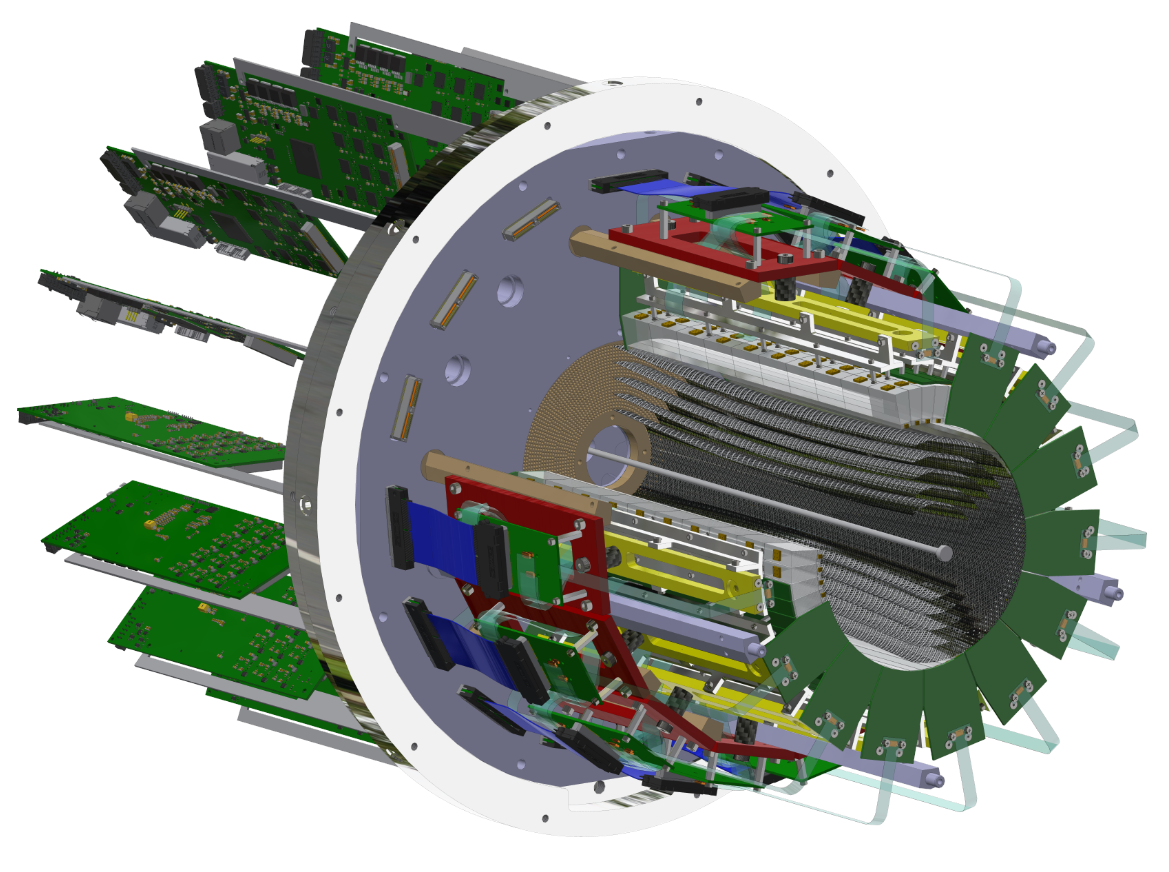
\includegraphics[width=0.4\linewidth]{figures/alert-full-assembly.png} & 
        %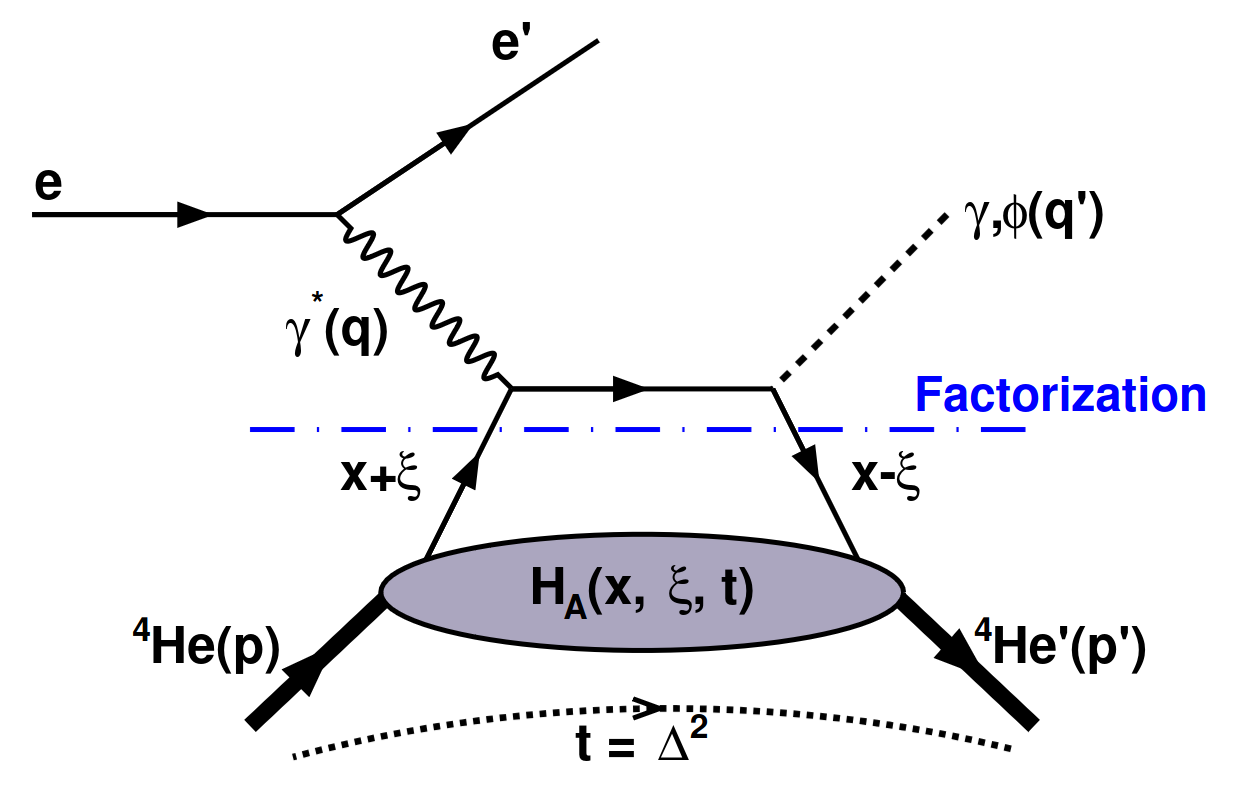
\includegraphics[width=0.4\linewidth, height=3.5cm]{figures/dvcs-feynman-diagram.png}
        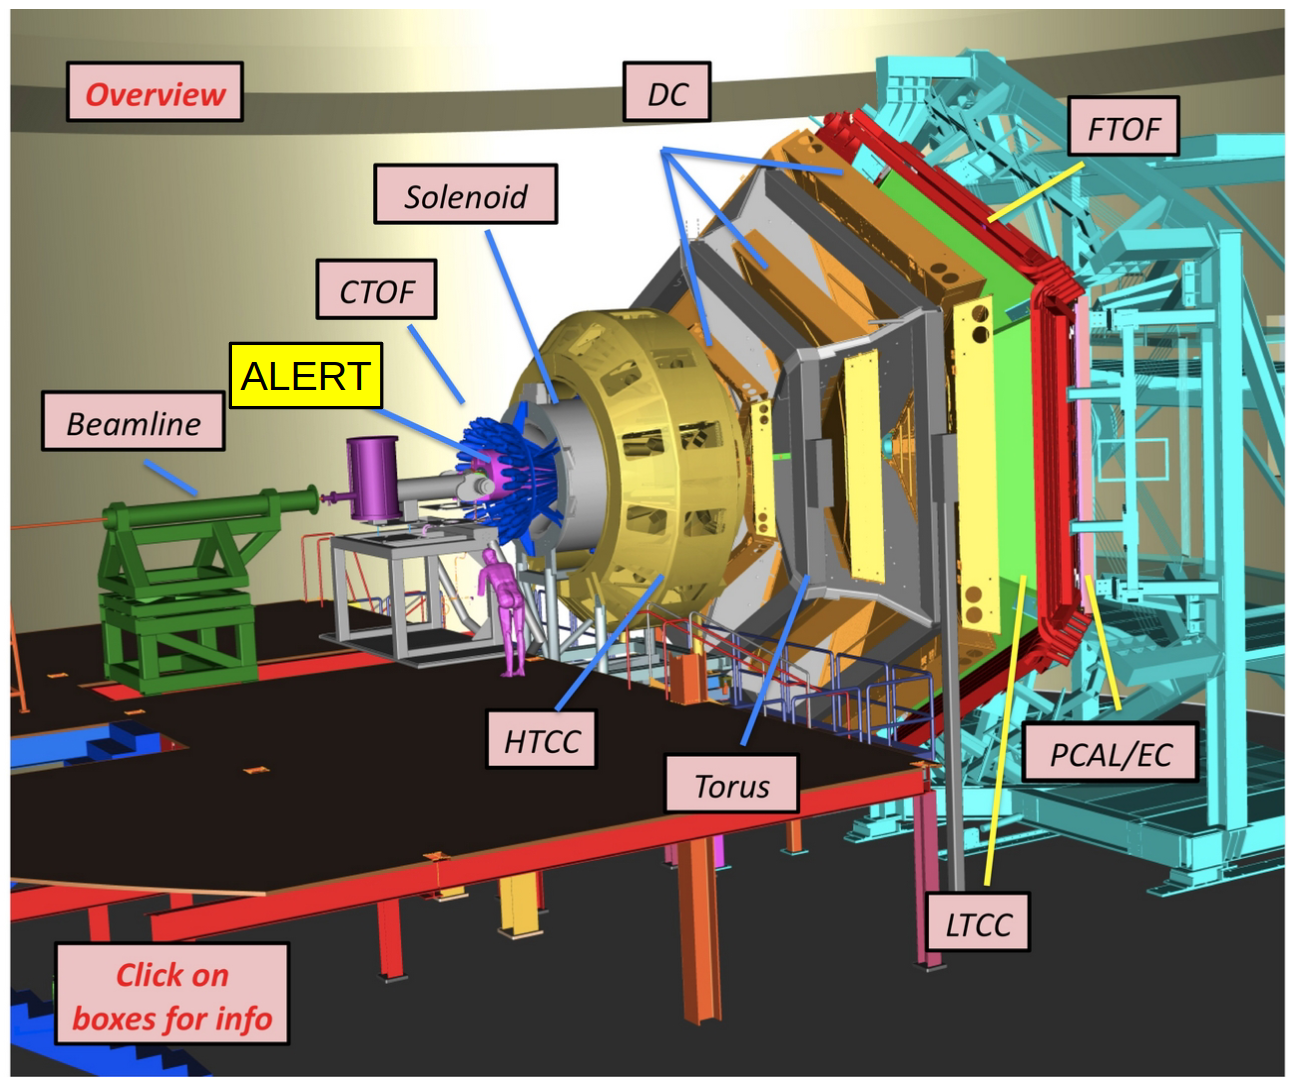
\includegraphics[width=4cm, height=3.4cm]{figures/clas12-with-alert.png}
    \end{tabular}
    
\end{frame}

\begin{frame}{ALERT Hyperbolic Drift Chamber (AHDC)}
    \begin{itemize}
        \item Cylindrical wire chamber filled with He4/CO$_2$ (80/20)
        \item Novelty : 
            \begin{itemize}
                \item All wires have the same $\diameter$, 30 µm, and AlMg5 material
                \item Total of 3026 wires, 576 are readouts with positive charge
                %\item No guard wires (sense wire $\leftrightarrow$ HV, field wire $\leftrightarrow$ ground)
                \item Superlayer structure : 3-5-5-5-3, resulting in 8 detection layers
                \item It has stereo angles varying from 3.8$^\circ$ to 7.4$^\circ$ between superlayer for the vz reconstruction
            \end{itemize}
        \item Use the DREAM electronics developed at CEA
    \end{itemize}

    \centering
    \vspace{0.4cm}

    %\includegraphics[width=0.35\linewidth]{figures/build/ahdc-cell.pdf}
    \begin{tabular}{cc}
        \includegraphics[width=0.32\linewidth]{figures/build/ahdc-cell.pdf} & 
        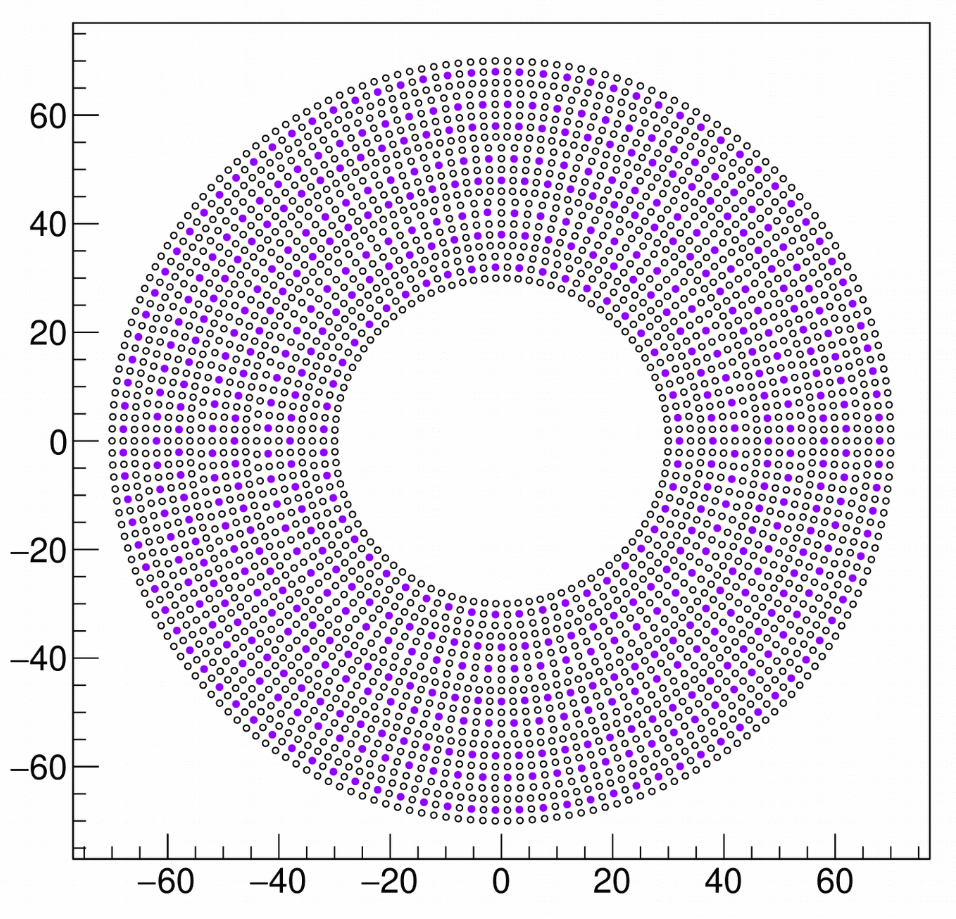
\includegraphics[width=4cm, height=3.8cm]{figures/all-ahdc-wires.png}
    \end{tabular}
\end{frame}

\begin{frame}{ALERT during the run period}
    \begin{itemize}
        %\item AHDC Assembly time : 3 months
        %\item Use the DREAM electronics developed at CEA
        \item The detector ran successfully during 5 months of data taking (from April 2025 to September 2025)
        %\item Running condition:
             
    \end{itemize}

    \begin{center}
        % \begin{minipage}{0.45\linewidth}
        %     \begin{itemize}
        %         \item[$\circ$] HV $\sim$ 1400-1500 V
        %         \item[$\circ$] Event rate $\sim$ 10 kHz
        %         \item[$\circ$] $6.42 \times 10^{10}$ trigger events collected
        %     \end{itemize}
        % \end{minipage}
        % \begin{minipage}{0.45\linewidth}
        %     \begin{itemize}
        %         \item[$\circ$] beam current up to 325 nA
        %         \item[$\circ$] nb. samples per WF : 20
        %         \item[$\circ$] sampling window $\sim 1$ µs
        %     \end{itemize}
        % \end{minipage}
        \begin{tabular}{ll}
            $\circ$ HV $\sim$ 1400-1500 V & $\circ$ beam current up to 325 nA\\
            $\circ$ Event rate $\sim$ 10 kHz & $\circ$ nb. samples per WF : 20\\
            $\circ$ $6.42 \times 10^{10}$ trigger events collected & $\circ$ sampling window $\sim 1$ µs\\
        \end{tabular}
    \end{center}
    

    \centering
    \vspace{0.5cm}

    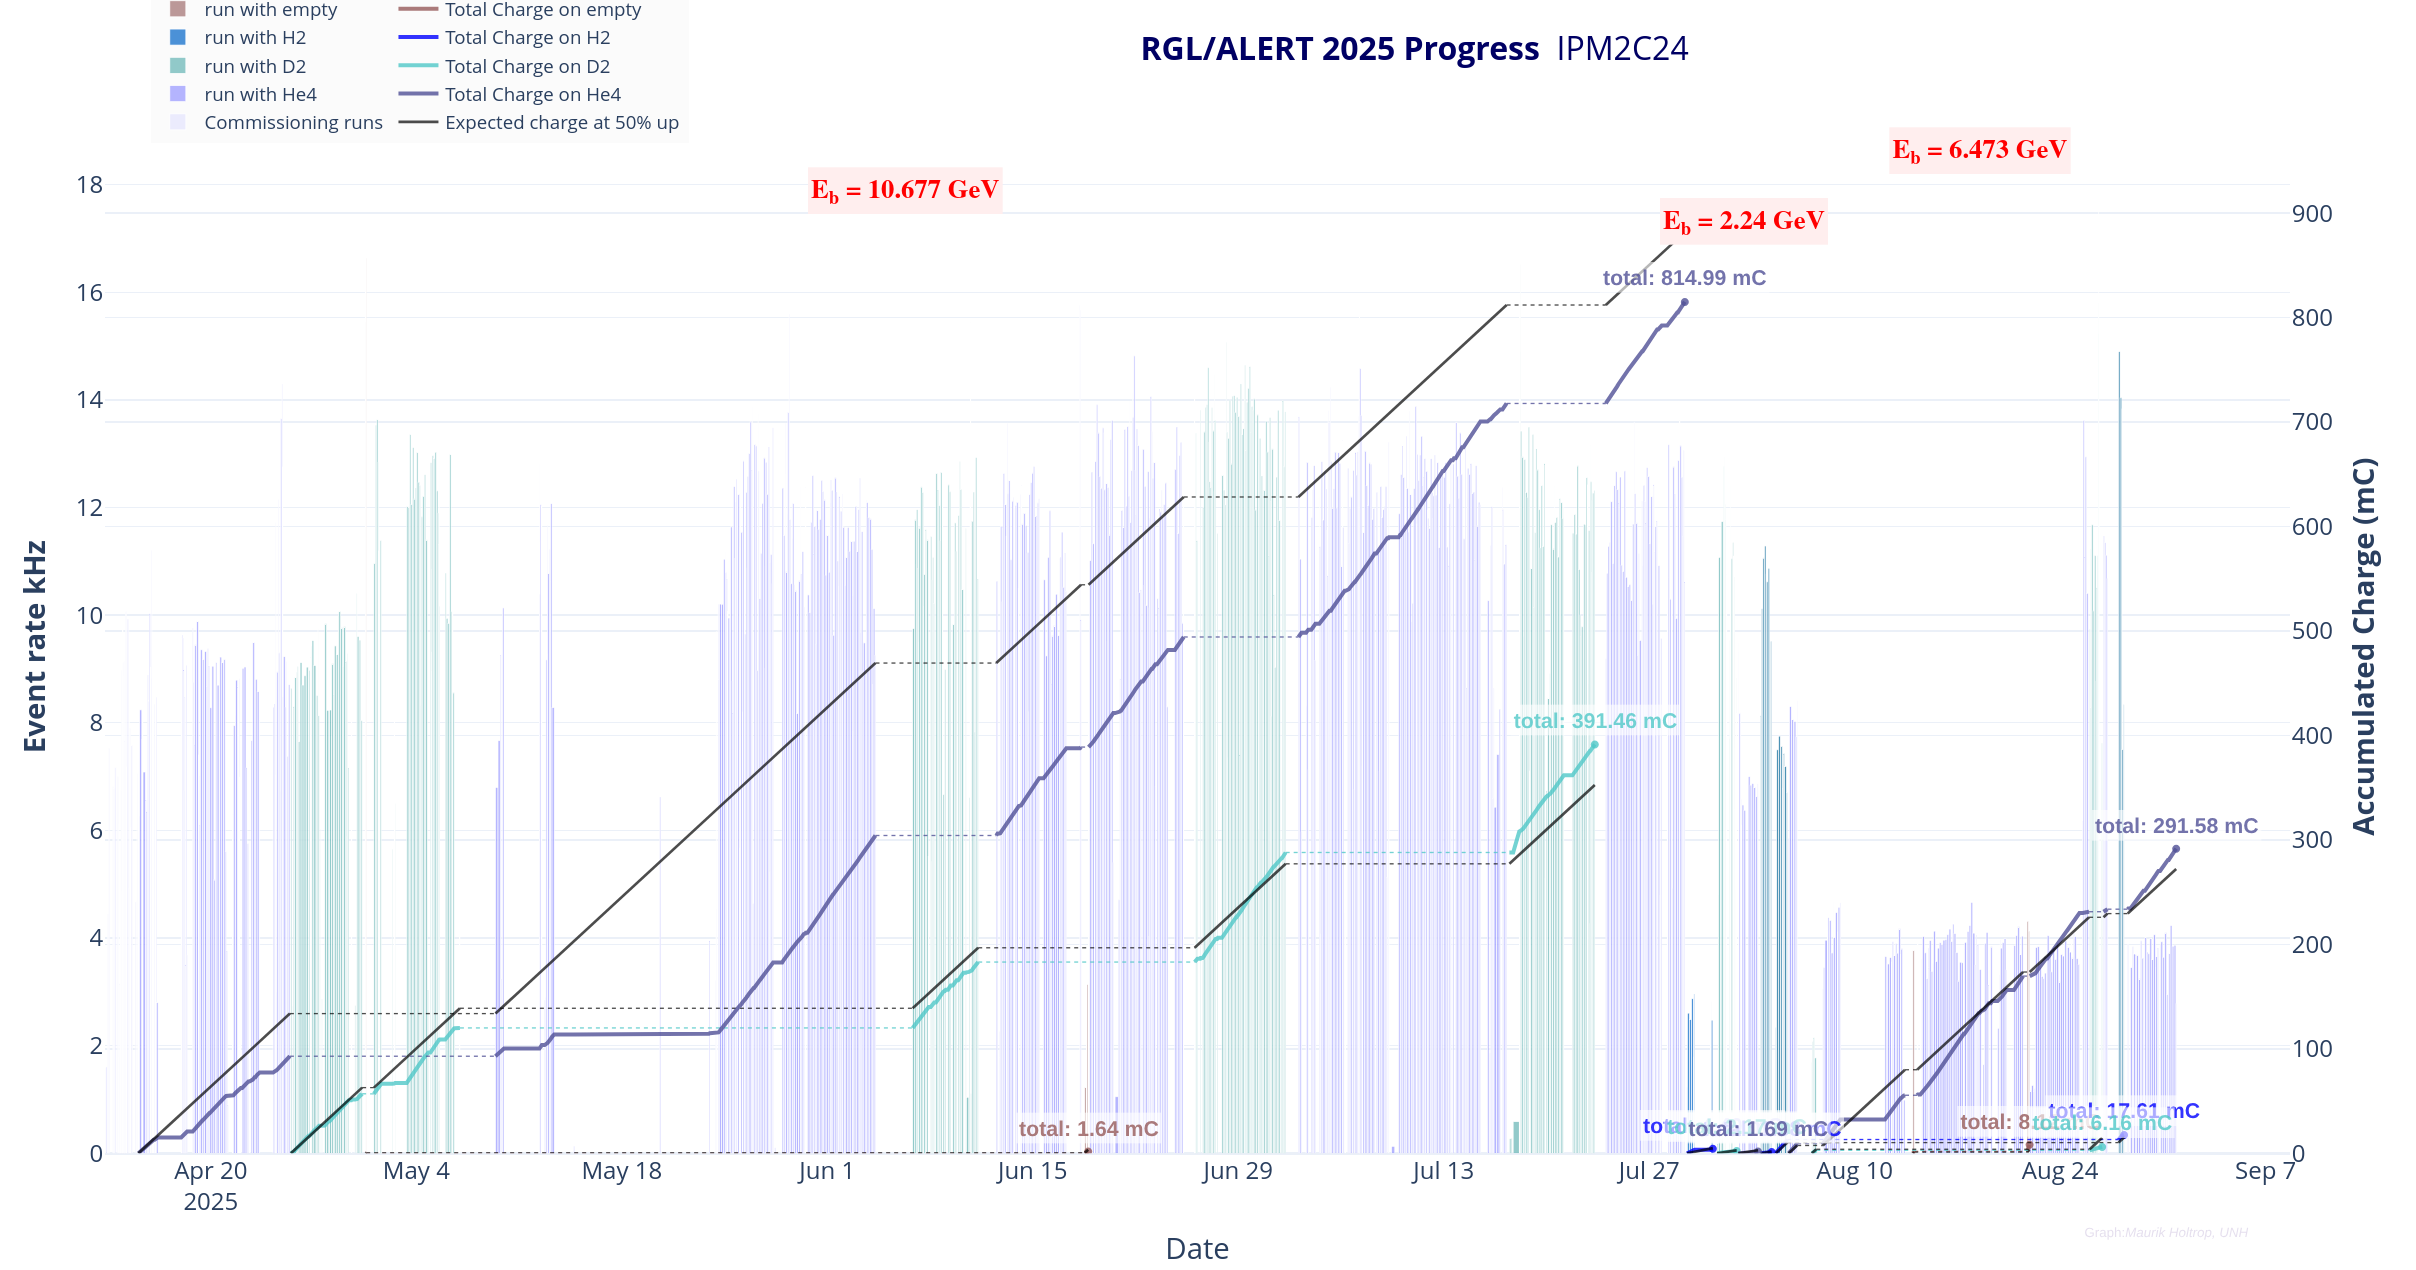
\includegraphics[width=0.75\linewidth]{figures/accumluted-charges.png}

\end{frame}

\begin{frame}{Assembly and transport}
    \begin{itemize}
        \item Assembly time : 3 months (last wire mounted on March 1, 2024 \footnote{My first day at IJCLab})
        \item Detector fully assembled in IJCLab and transported to JLab by plane wihout any issue
    \end{itemize}

    \centering
    \vspace{0.2cm}

    %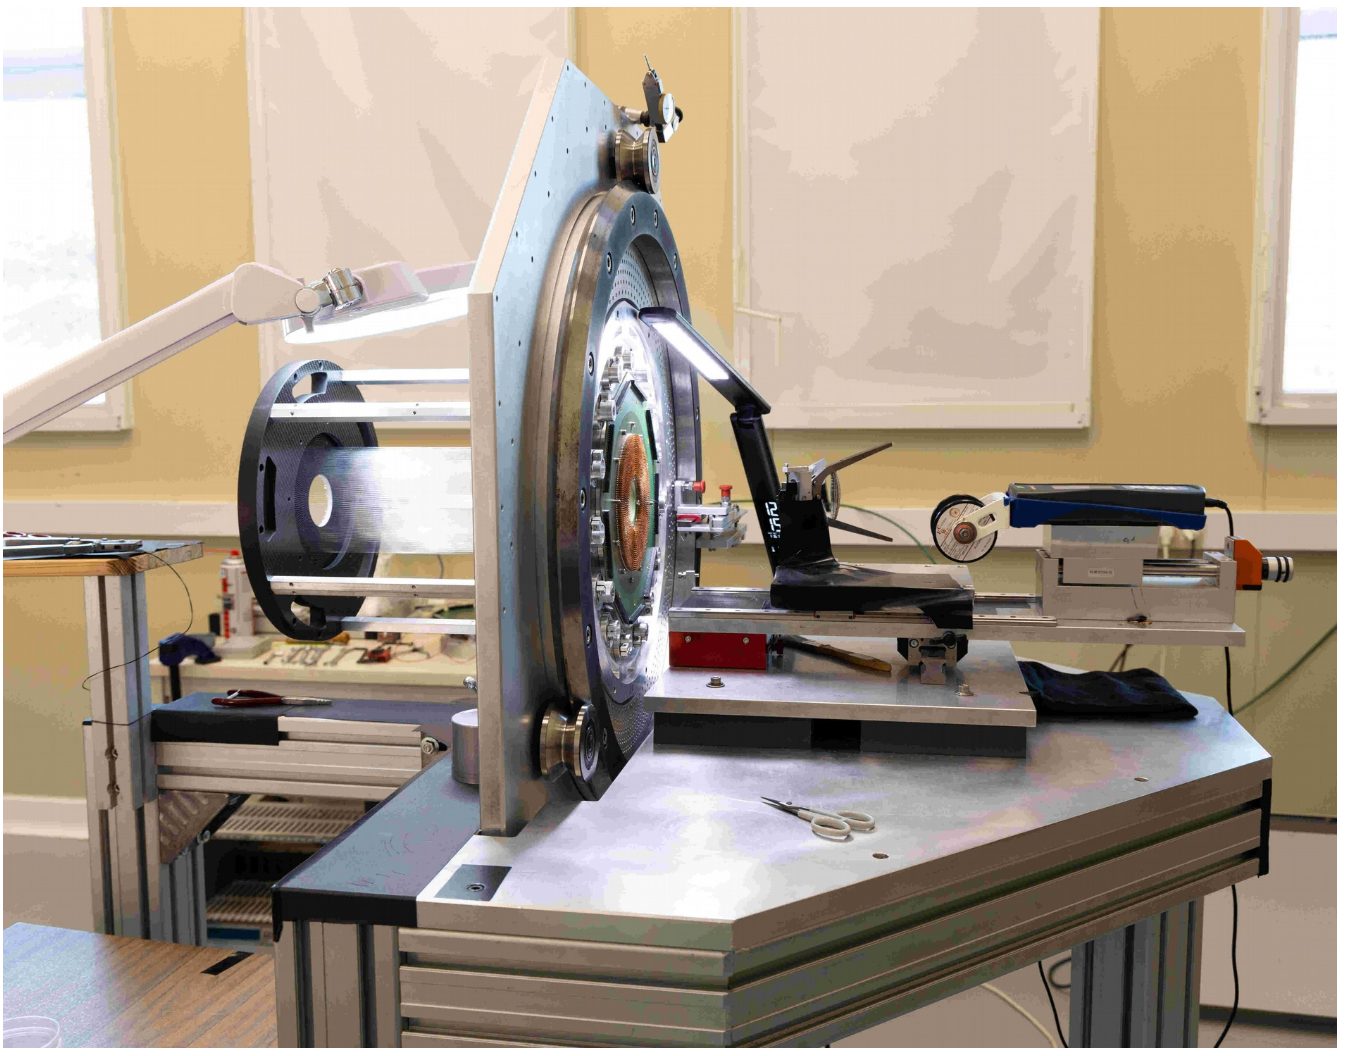
\includegraphics[width=0.4\linewidth]{figures/ahdc-during-assembly.png}
    \begin{tabular}{cc}
        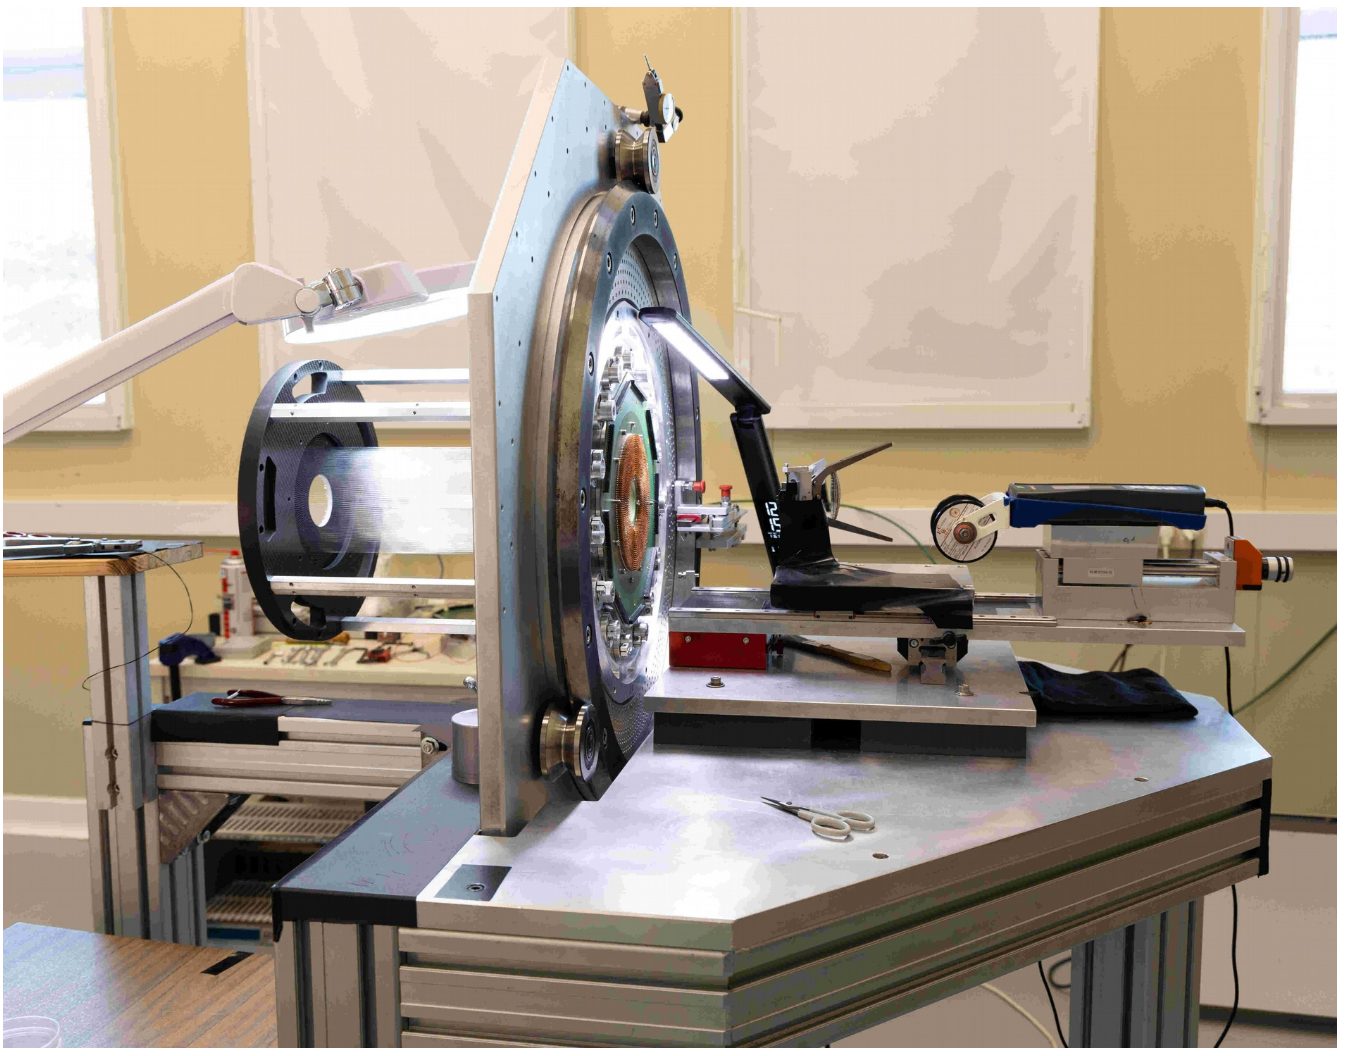
\includegraphics[width=0.4\linewidth]{figures/ahdc-during-assembly.png} & 
        picture of the box in the plane
    \end{tabular}
\end{frame}

\begin{frame}{Hit selection}
    \begin{itemize}
        \item First step of the AHDC reconstruction software
        \item On average, we have 20-40 \% occupancy on the first layer of the AHDC
        \item The noise presents a clear pattern that make it possible to classify hits into 7 categories (wfType 6 to 0)
        \item Good hits are those with wfType $\leq$ 2 and within a calibrated time window
    \end{itemize}

    \centering
    \vspace{0.2cm}

    % file : rec-data-r22712-v143 evt 143
    \begin{figure}
        \begin{subfigure}{0.4\linewidth}
            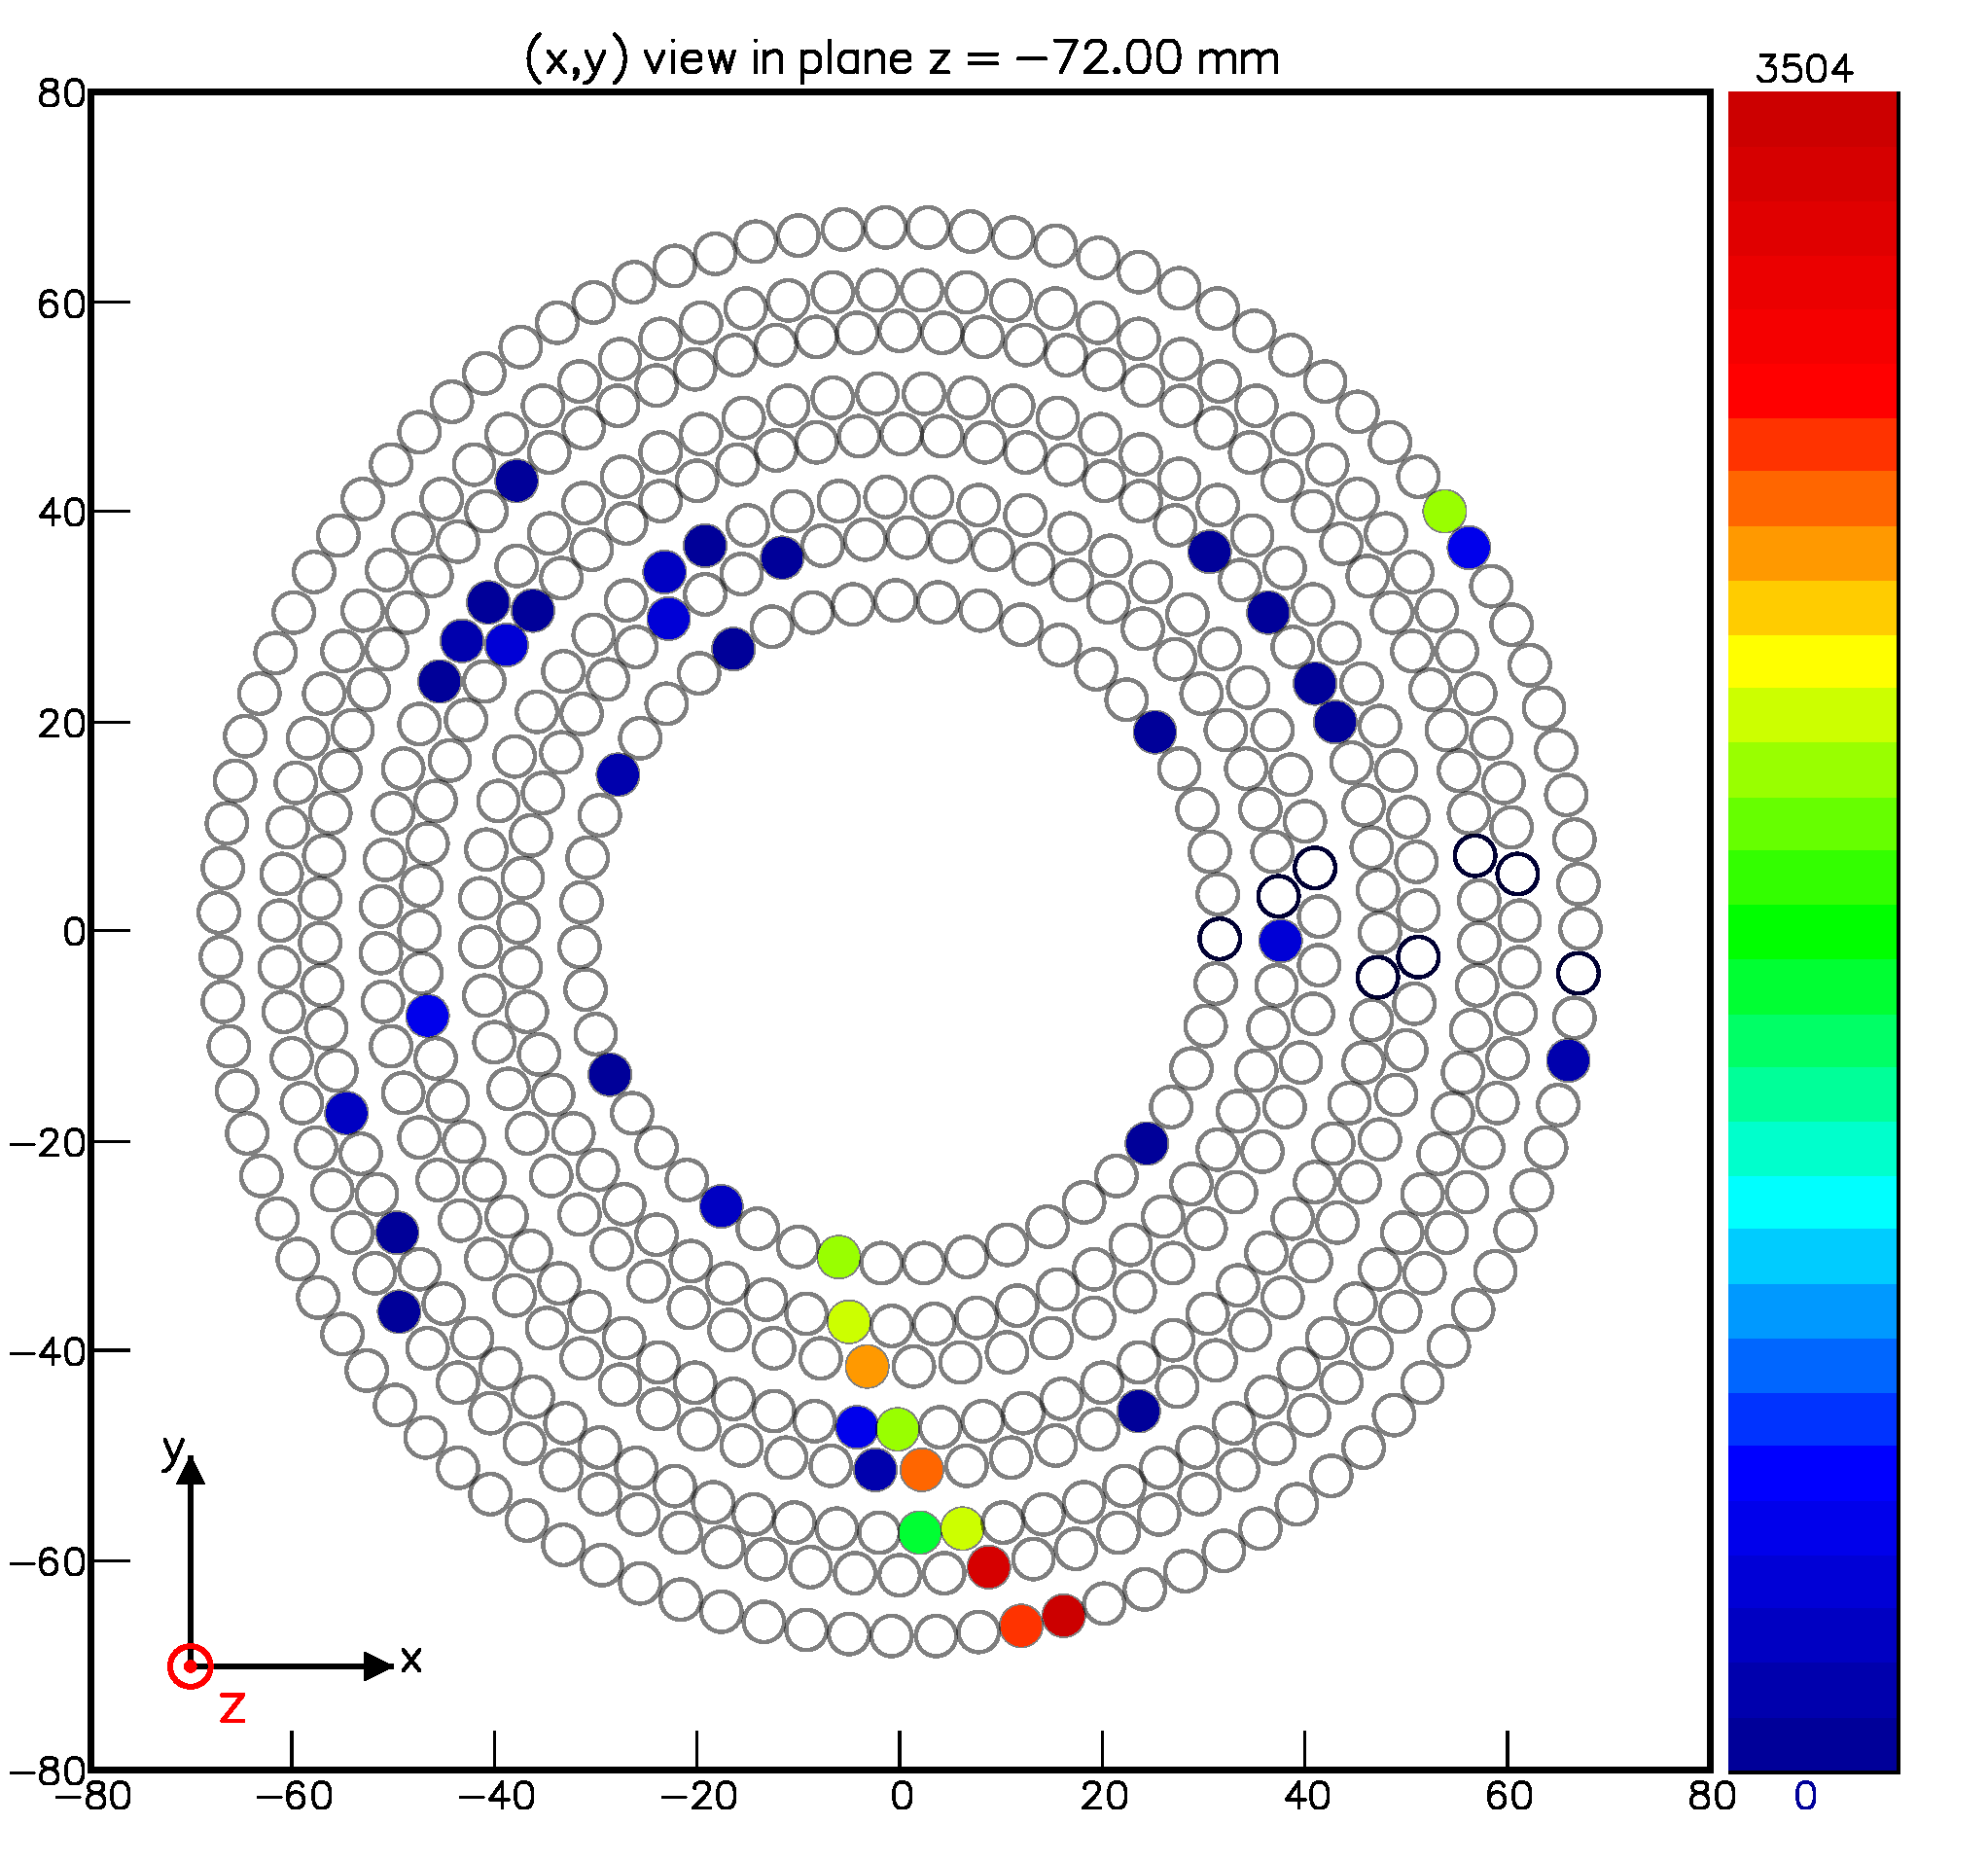
\includegraphics[width=\linewidth]{figures/event-display-no-cleaning.pdf}
            \caption{All hits}
        \end{subfigure}
        \hspace{0.2cm}
        \begin{subfigure}{0.4\linewidth}
            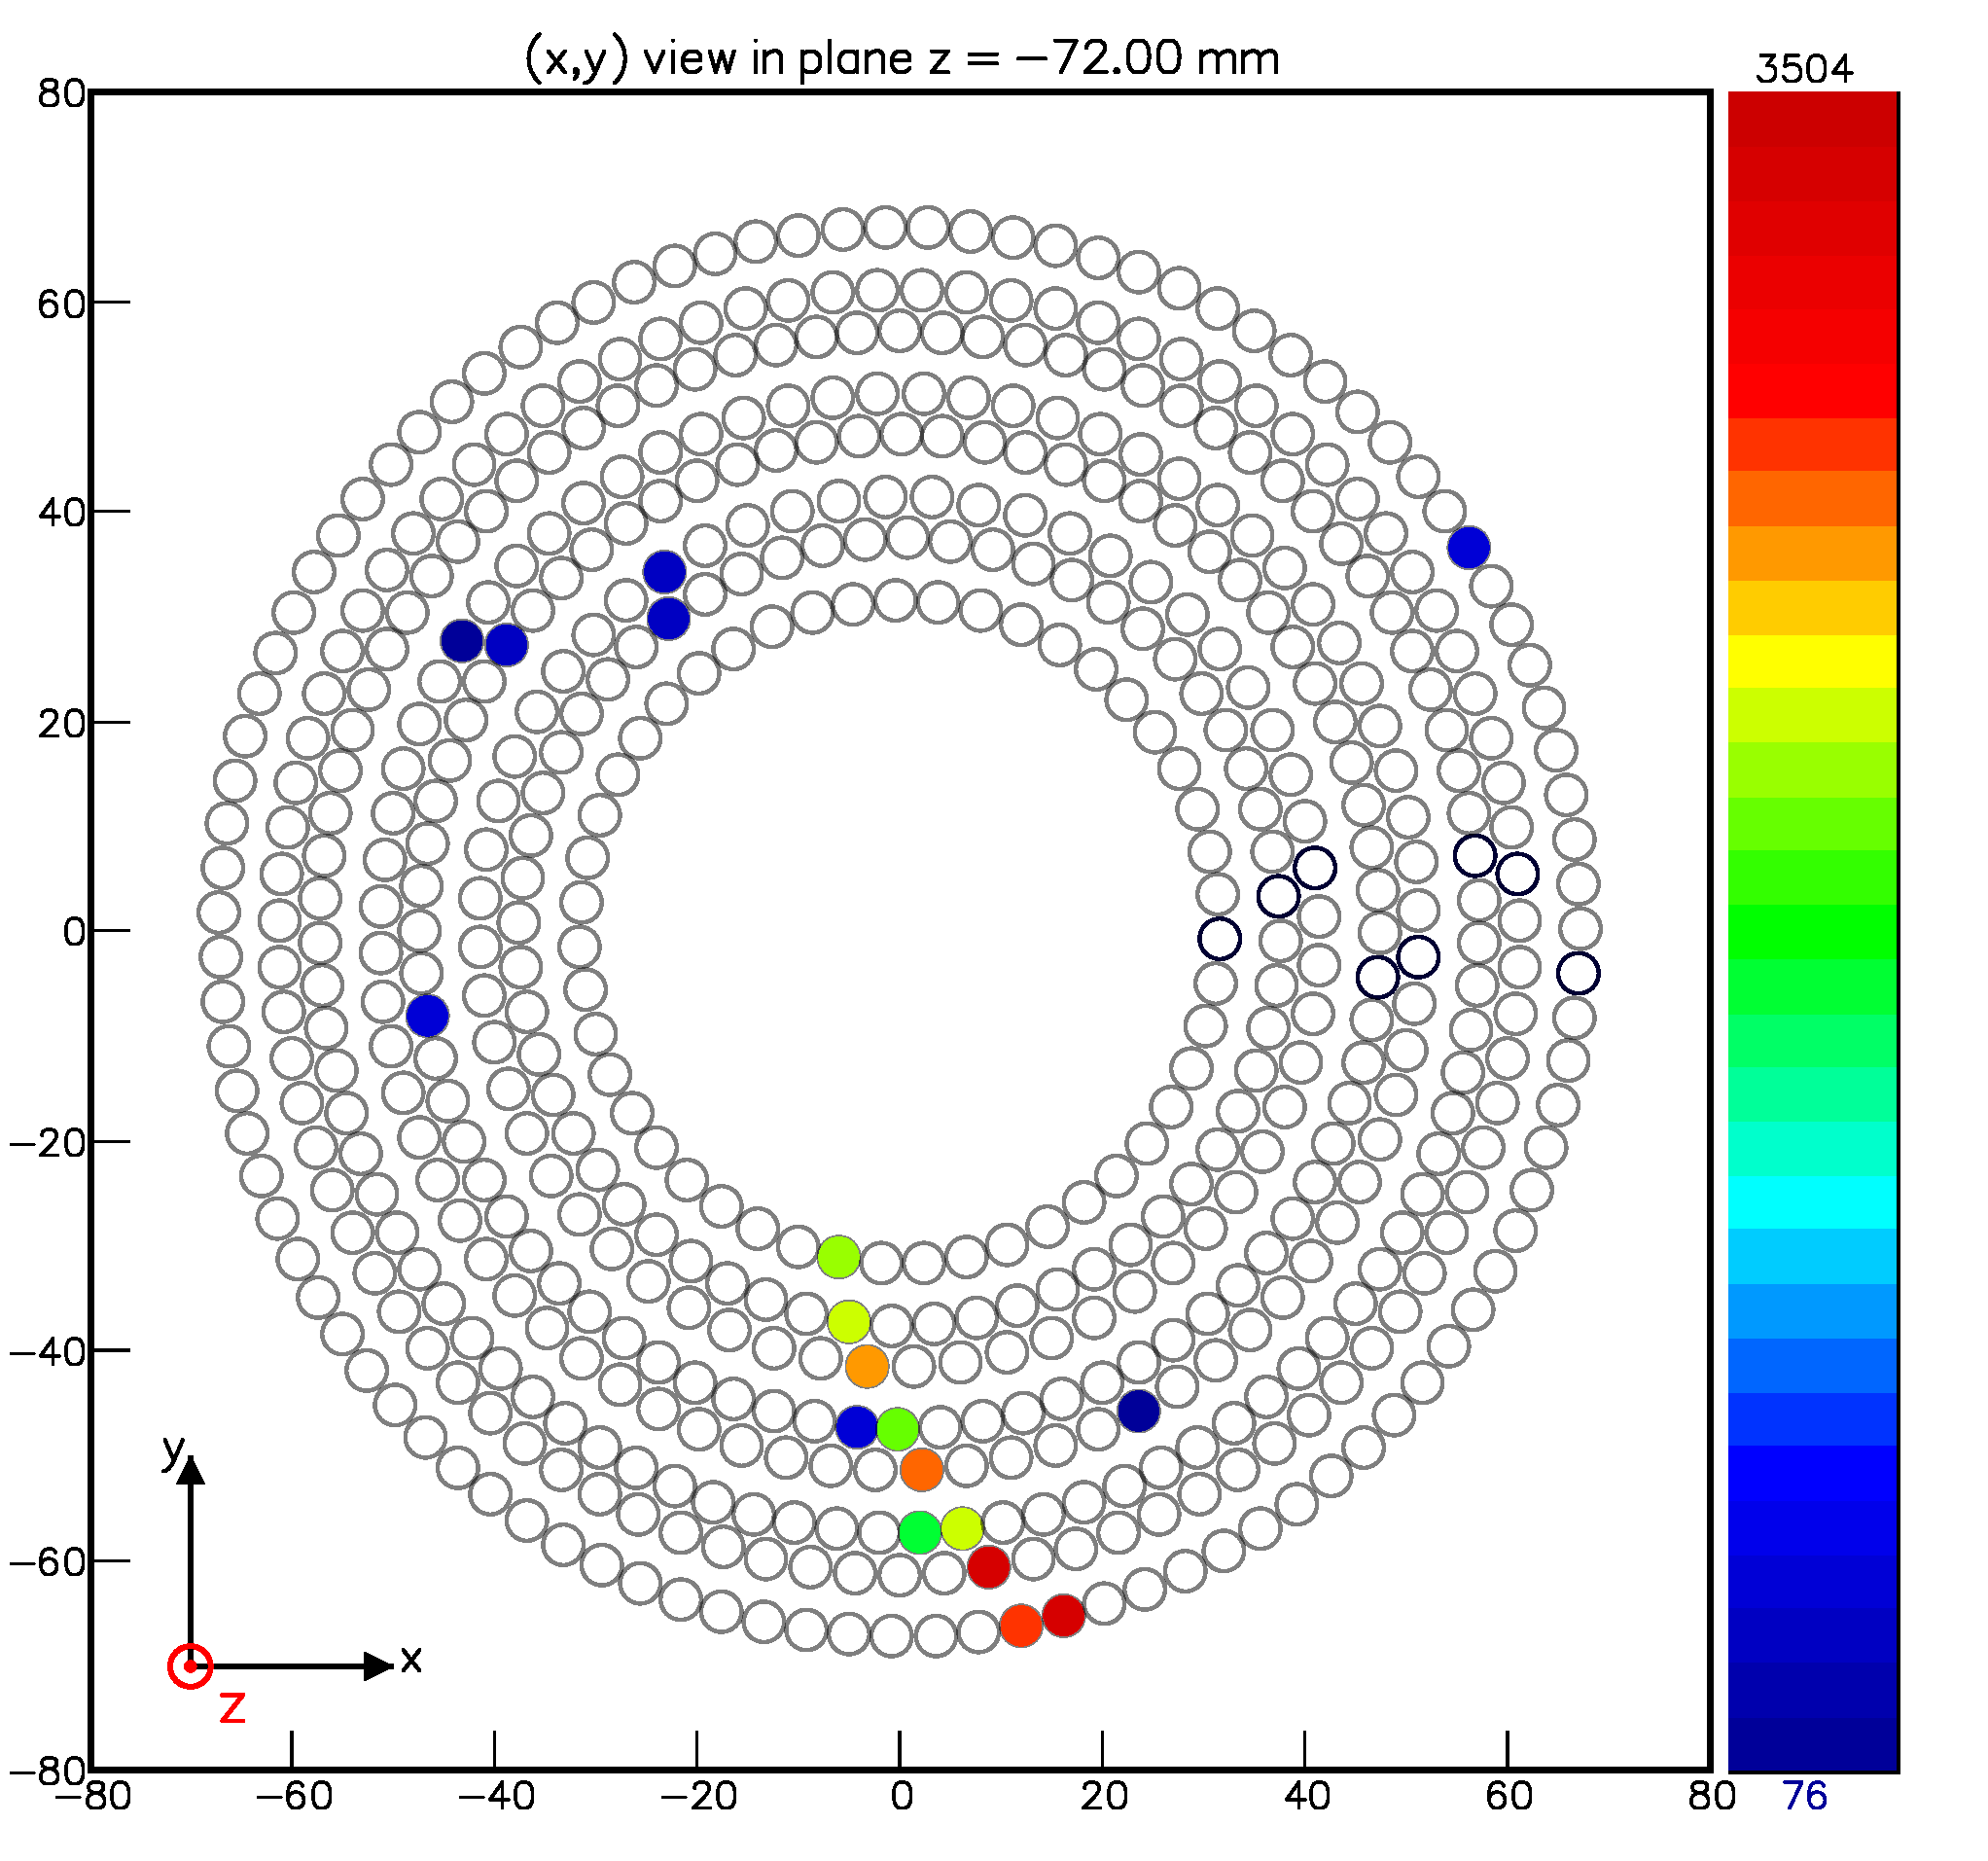
\includegraphics[width=\linewidth]{figures/event-display-cleaning.pdf}
            \caption{Only hits passing the selection cuts}
        \end{subfigure}
        \vspace{-8pt}
        \caption{Typical event display in the AHDC}
    \end{figure}
\end{frame}

% \begin{frame}{AHDC track reconstruction}
%     \begin{itemize}
%         \item fjgjgkskkm
%     \end{itemize}

%     \centering
%     \vspace{0.2cm}

%     \includegraphics[width=0.7\linewidth]{figures/build/ahdc-atof-hits.pdf}
% \end{frame}

\begin{frame}{Waveform classification}
    \begin{itemize}
        \item We consider that good hits have wfType $\leq 2$
    \end{itemize}

    \centering
    \vspace{0.2cm}

    { \footnotesize
        \begin{tabular}{ll} 
            $\circ$ wfType 6 $\rightarrow$ too short (nsamples $\leq$ 10) & $\circ$ wfType 2 $\rightarrow$ bad
    trailingEdgeTime \\
            $\circ$ wfType 5 $\rightarrow$ decreasing baseline & $\circ$ wfType 1 $\rightarrow$ saturating\\
            $\circ$ wfType 4 $\rightarrow$ bad ToT (ToT $<$ 300) & $\circ$ wfType 0 $\rightarrow$ OK\\
            $\circ$ wfType 3 $\rightarrow$ pileup but classified as 2& \\
        \end{tabular}
    }

    \begin{itemize}
        \item The occupancy drops at 7 \% in the first layer 
        \item Additional cuts based on the calibrated times are added before entering the Track Finder
    \end{itemize}

    \vspace{0.2cm}
    
    { \setlength{\tabcolsep}{1pt}
        \begin{tabular}{llll}
            
\includegraphics[width=0.24\linewidth]{figures/wfType6.pdf} & 
                
\includegraphics[width=0.24\linewidth]{figures/wfType5.pdf} & 
                    
\includegraphics[width=0.24\linewidth]{figures/wfType4.pdf} &
                        
\includegraphics[width=0.24\linewidth]{figures/wfType3.pdf} \\  
            
\includegraphics[width=0.24\linewidth]{figures/wfType2.pdf} & 
                
\includegraphics[width=0.24\linewidth]{figures/wfType1.pdf} & 
                    
\includegraphics[width=0.24\linewidth]{figures/wfType0.pdf} & 
                        \includegraphics[width=2.5cm,height=1.5cm]{figures/build/legend-wfType.pdf} \\
        \end{tabular}
    }
    %Examples of waveforms with different waveform types 
\end{frame}

\begin{frame}{Track Finder}
    \begin{itemize}
        \item ...
    \end{itemize}

    \centering
    \vspace{0.2cm}

    %Waveform types to be added
\end{frame}

\begin{frame}{Kalman Filter}
    \begin{itemize}
        \item ...
    \end{itemize}

    \centering
    \vspace{0.2cm}

    %Waveform types to be added
\end{frame}

\begin{frame}{AHDC resolution}
    \begin{itemize}
        \item Residuals
    \end{itemize}

    \centering
    \vspace{0.2cm}

    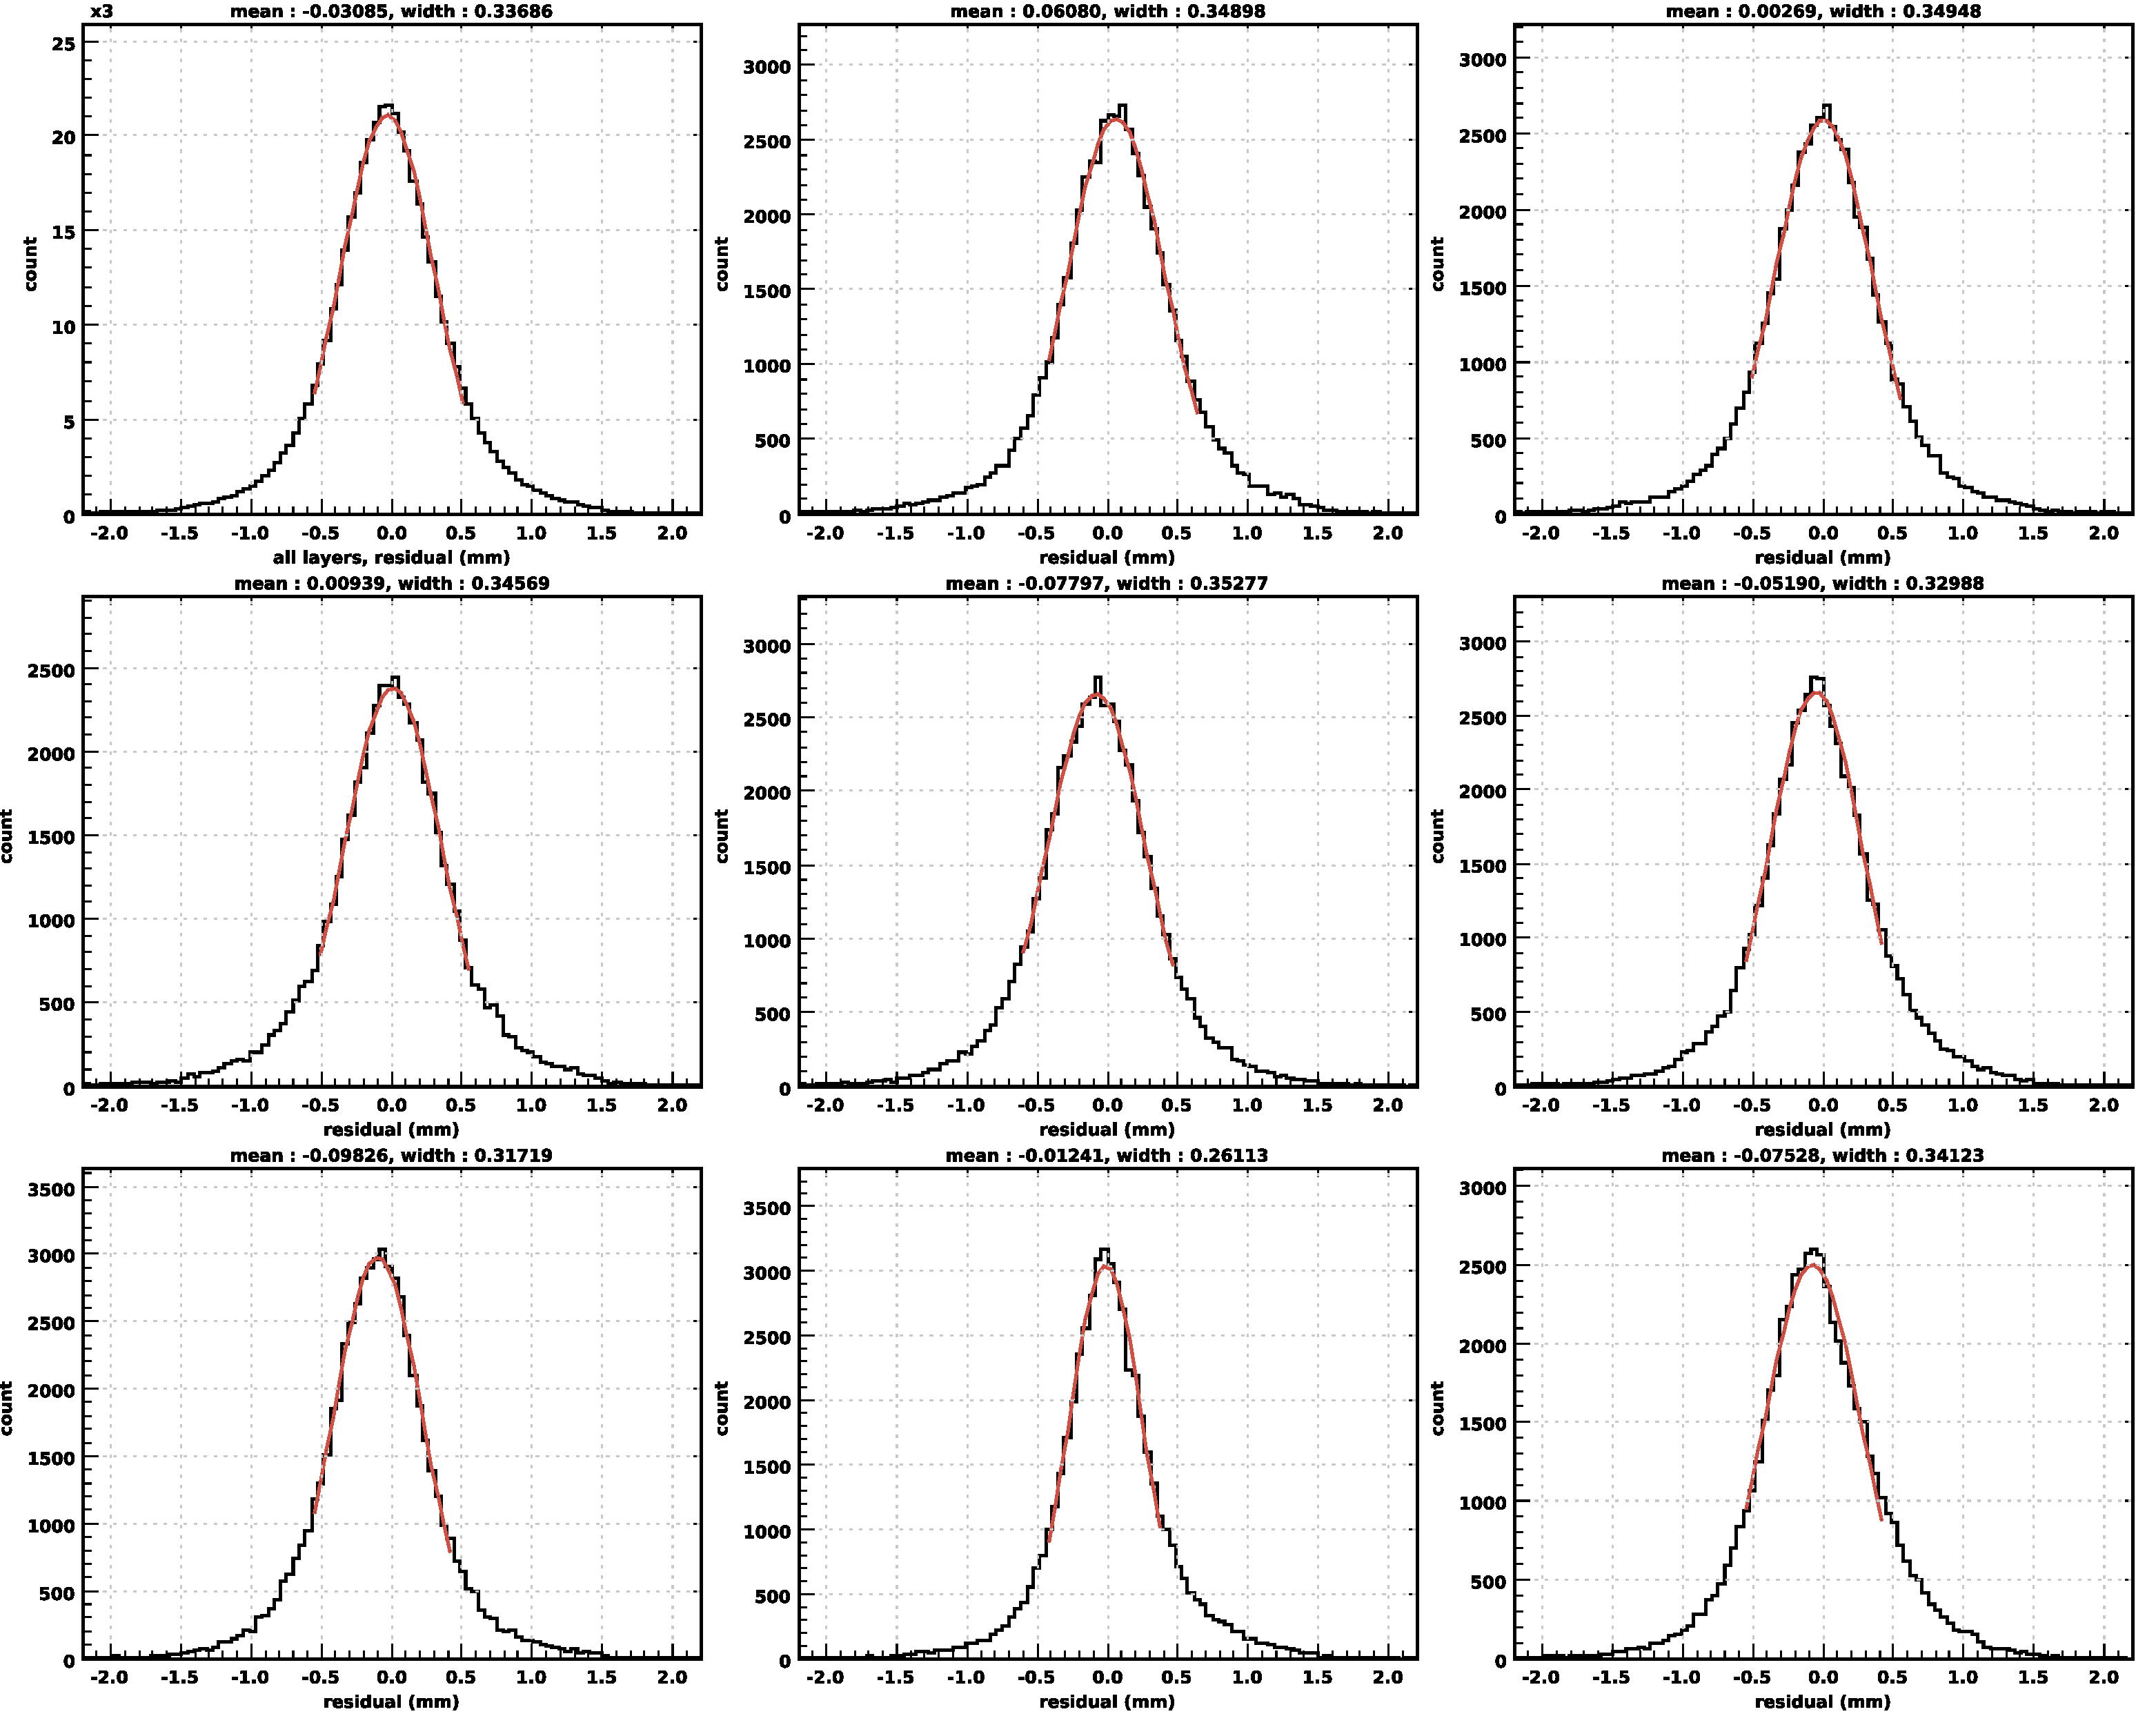
\includegraphics[width=0.7\linewidth]{figures/residual_normal_iter_1.pdf}
\end{frame}

\begin{frame}{AHDC resolution}
    \begin{itemize}
        \item Time2distance
    \end{itemize}

    \centering
    \vspace{0.2cm}

    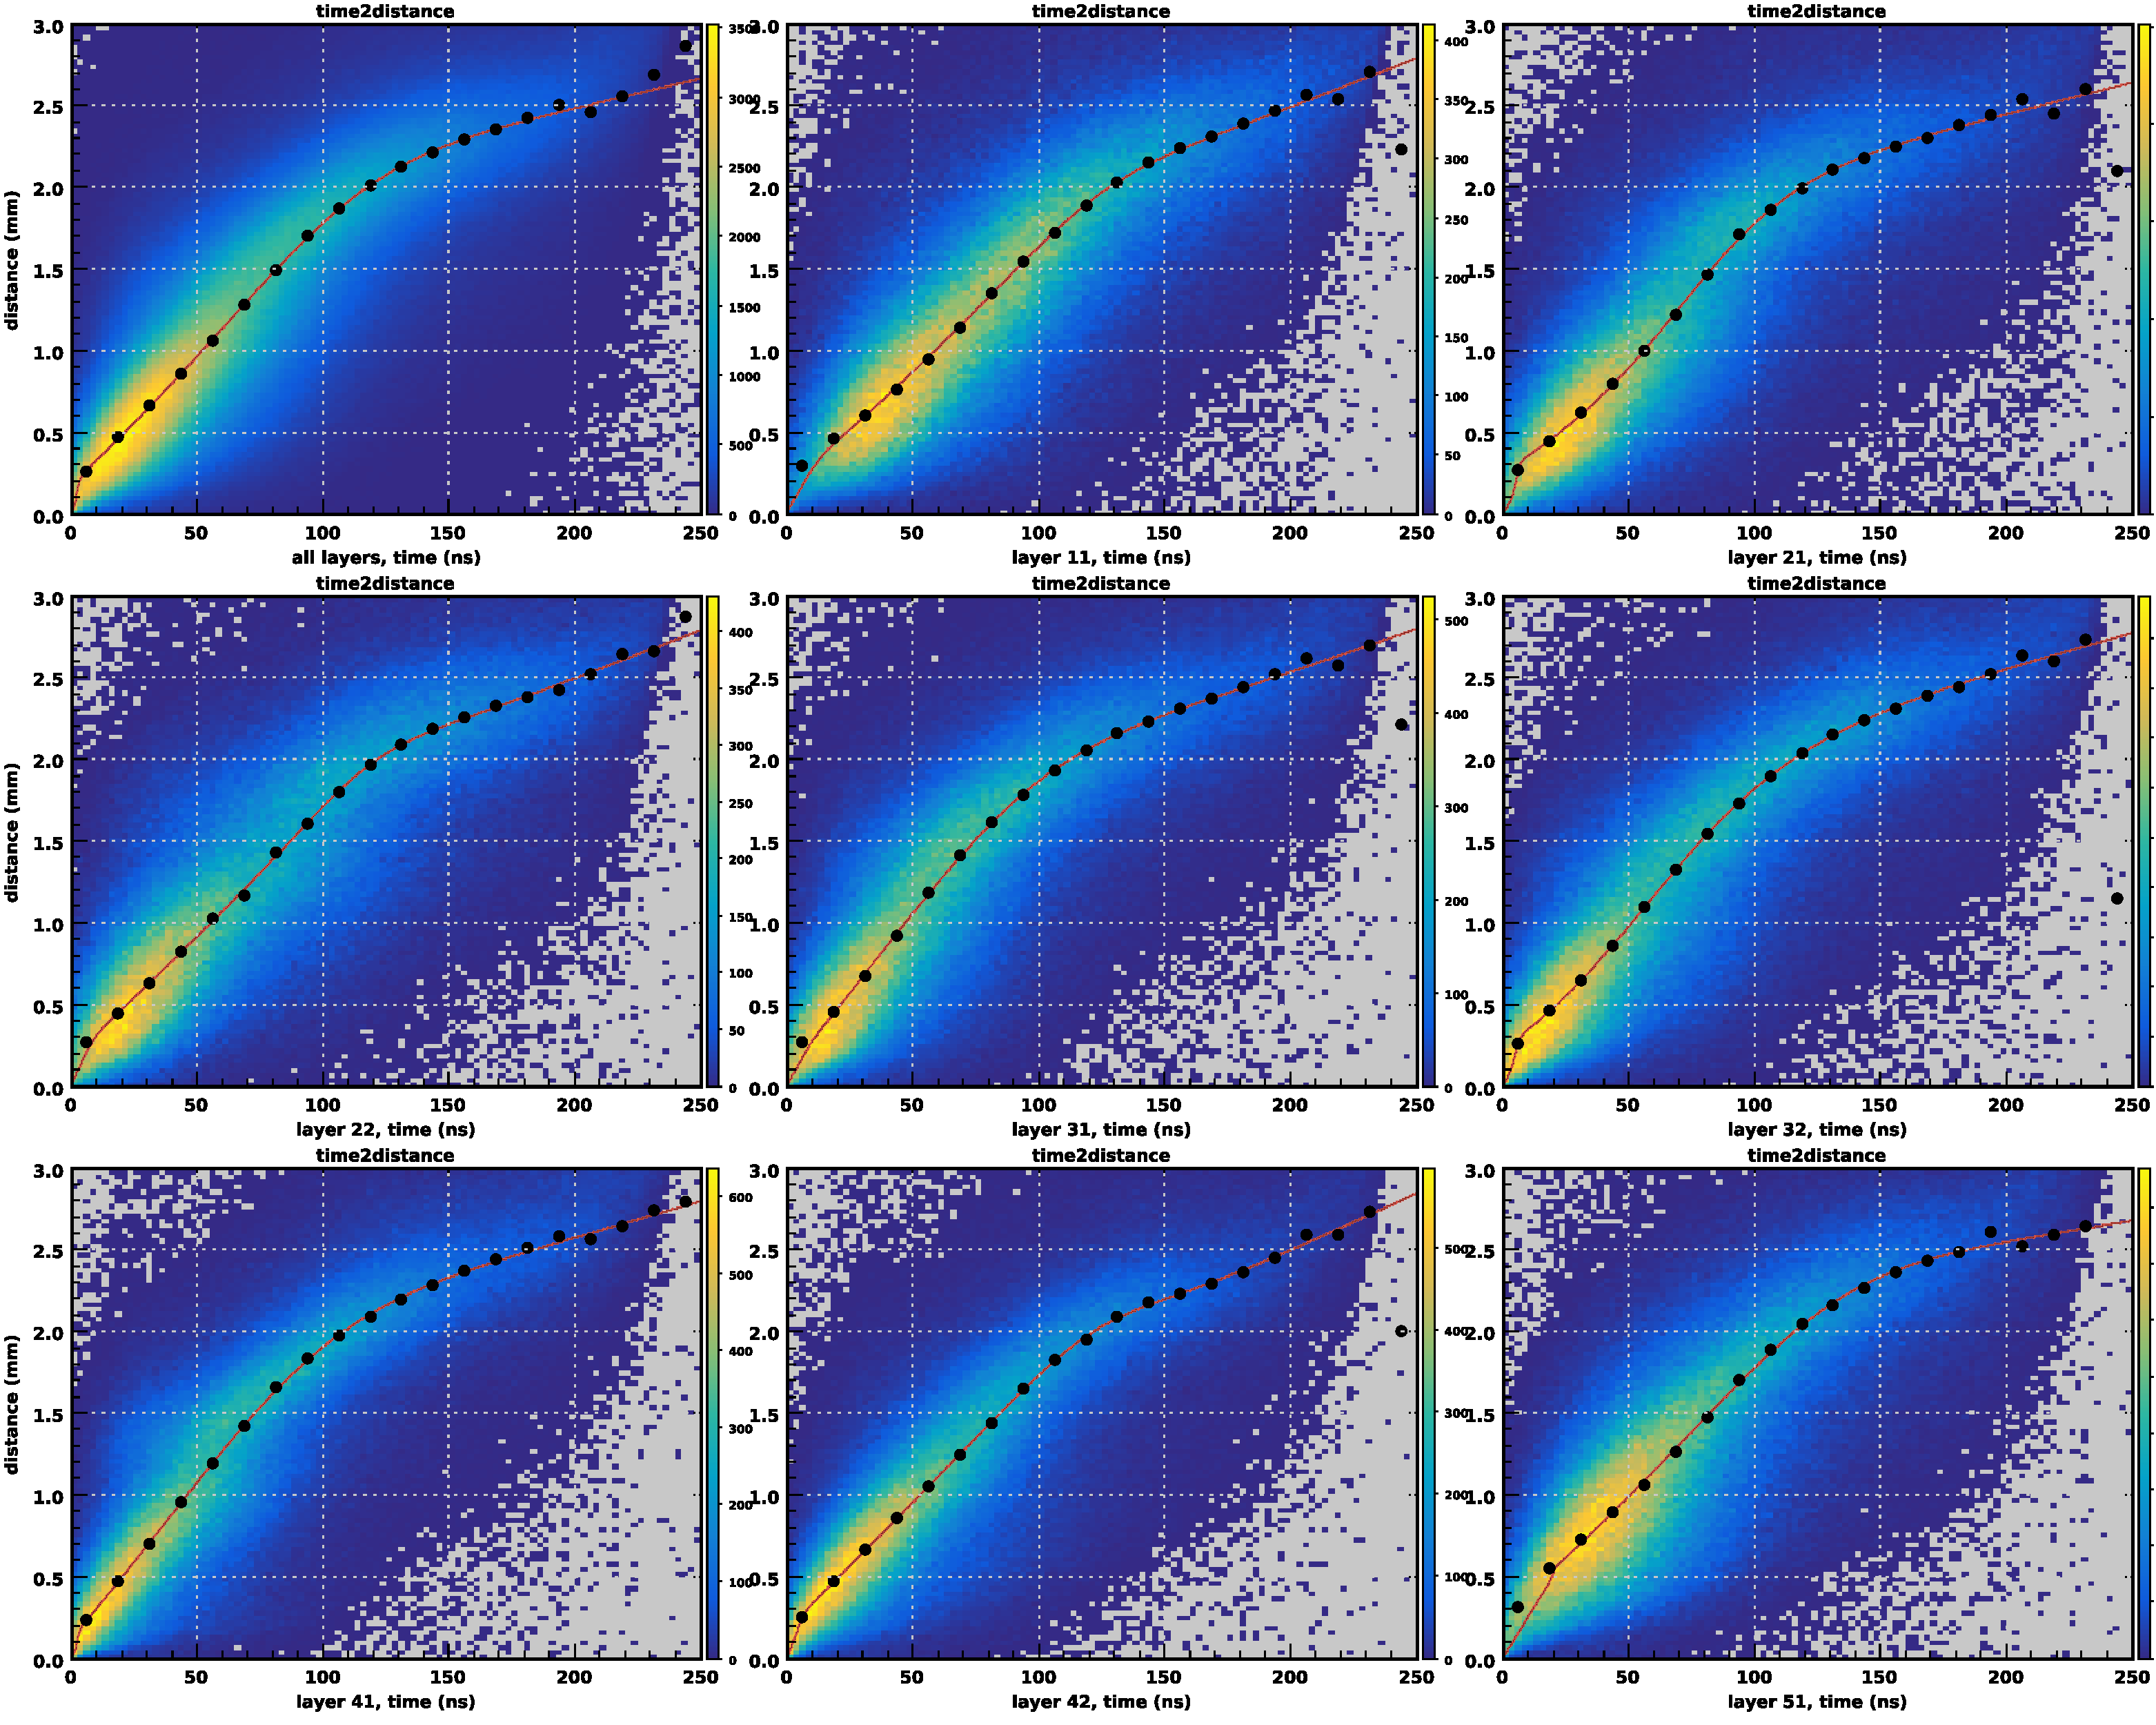
\includegraphics[width=0.7\linewidth]{figures/time2distance_iter_1_after_as_limitation.pdf}
\end{frame}

\begin{frame}{Particle identification}
    \begin{itemize}
        \item gggggfff
    \end{itemize}

    \centering
    \vspace{0.2cm}

    
\includegraphics[width=0.7\linewidth]{figures/recon-status-dEdx-versus-momentum.pdf}
\end{frame}






\end{document}


